\documentclass{article}

\usepackage{caption}
\usepackage{subcaption}
\usepackage{graphicx}
\usepackage{tikz}
\usepackage{tikzsymbols}
\usetikzlibrary{calc}
\usepackage{float}
\usepackage{pdflscape}
\usepackage{geometry}
\geometry{a4paper, landscape, margin=1cm}


\def\centerarc[#1](#2)(#3:#4:#5){\draw[#1] ($(#2)+({#5*cos(#3)},{#5*sin(#3)})$) arc (#3:#4:#5);}


\pagestyle{empty}
\begin{document}
	\centering
	\begin{figure}[H]
		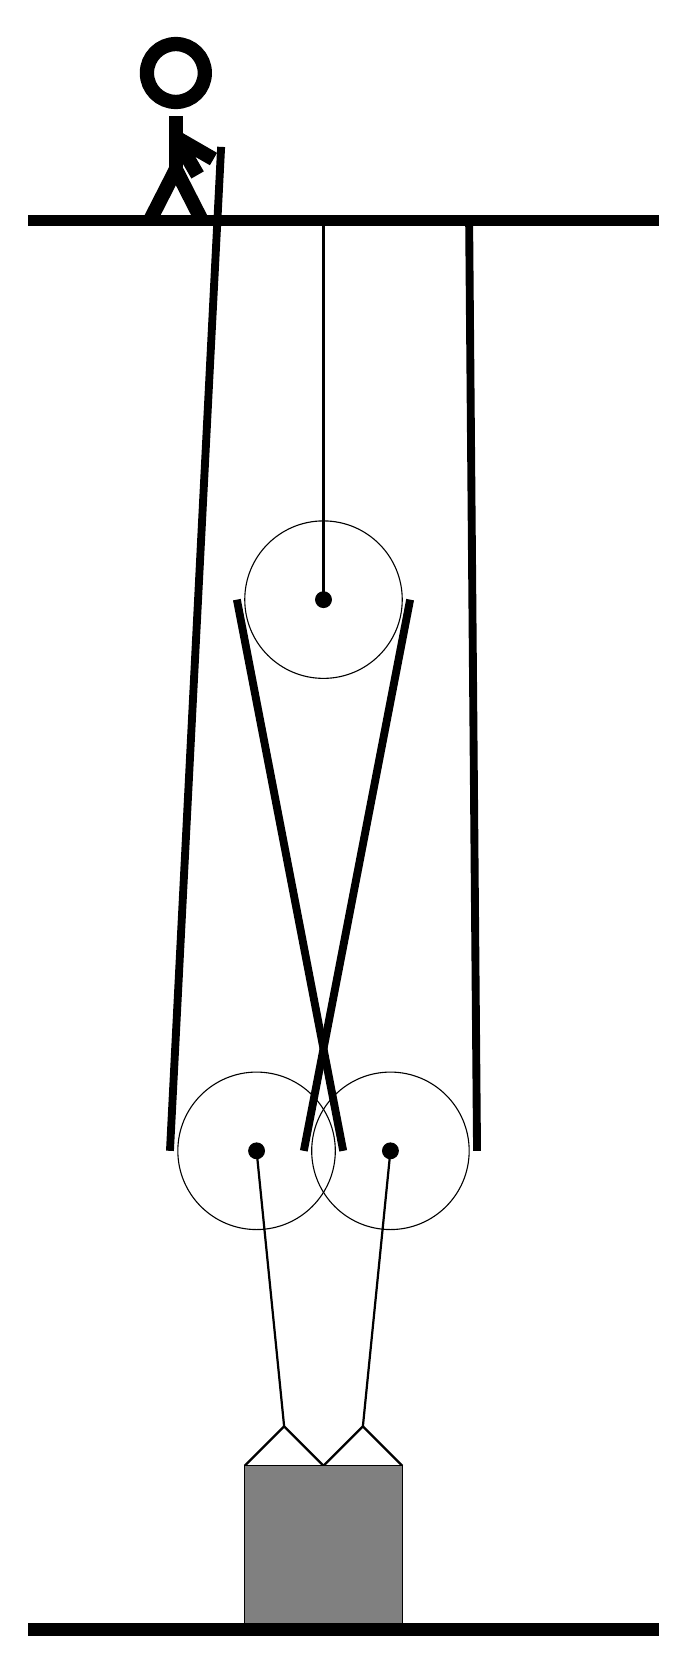
\begin{tikzpicture}
			%%%%% START %%%%%
			\def\a{14.75}
			\def\radlg{\radrp-0.1}
			\def\radrp{1.1}
			\def\radsm{0.1}
			\def\xone{0.9}
			\def\yone{3}
			\def\xtwo{1.75}
			\def\ytwo{10}
			\def\xthree{2.6}
			\def\ythree{3}
			\def\dx{-0.05}
			\def\dy{13}
			\def\hlen{11}
			\def\width{1mm}
			
			\draw[fill=black] (-2,\a) rectangle (6,\a+0.125);
			
			\draw (\xone,\yone) circle (\radlg);
			\draw[fill=black] (\xone,\yone) circle (\radsm);

			\draw (\xtwo,\ytwo) circle (\radlg);
			\draw[fill=black] (\xtwo,\ytwo) circle (\radsm);
			\draw[thick] (\xtwo,\ytwo) -- (\xtwo,\a);
			
			\draw (\xthree,\ythree) circle (\radlg);
			\draw[fill=black] (\xthree,\ythree) circle (\radsm);
		
			\draw[thick] (\xthree,\ythree) -- (\xtwo+0.5,\ytwo-\hlen+0.5);
			\draw[thick] (\xone,\yone) -- (\xtwo-0.5,\ytwo-\hlen+0.5);
			\draw[thick]  (\xtwo-1,\ytwo-\hlen) -- (\xtwo-0.5,\ytwo-\hlen+0.5) -- (\xtwo,\ytwo-\hlen);
			\draw[thick]  (\xtwo,\ytwo-\hlen) -- (\xtwo+0.5,\ytwo-\hlen+0.5) -- (\xtwo+1,\ytwo-\hlen);
			\draw[fill=black!50] (\xtwo-1,\ytwo-\hlen) rectangle (\xtwo+1,\ytwo-\hlen-2);
		
			\draw[line width=\width] (\dx+0.5,\a+1) -- (\xone-\radrp,\yone); 
			\centerarc[line width=\width](\xone,\yone)(180:360:\radrp);
			\draw[line width=\width] (\xone+\radrp,\yone) -- (\xtwo-\radrp,\ytwo);
			\centerarc[line width=\width](\xtwo,\ytwo)(0:180:\radrp);
			\draw[line width=\width](\xtwo+\radrp,\ytwo) -- (\xthree-\radrp,\ythree);
			\centerarc[line width=\width](\xthree,\ythree)(180:360:\radrp);
			\draw[line width=\width](\xthree+\radrp,\ythree) -- (\xthree+\radrp-0.1,\a);

			\node at (-0.07, \a+1.2) {\Strichmaxerl[10][120][-30]};
			
			\draw[fill=black] (-2,-3) rectangle (6,-3.15);
			%%%%% END %%%%%
		\end{tikzpicture}
	\end{figure}
	
\end{document}